\documentclass[14pt]{extbook}
\usepackage{multicol, enumerate, enumitem, hyperref, color, soul, setspace, parskip, fancyhdr} %General Packages
\usepackage{amssymb, amsthm, amsmath, latexsym, units, mathtools} %Math Packages
\everymath{\displaystyle} %All math in Display Style
% Packages with additional options
\usepackage[headsep=0.5cm,headheight=12pt, left=1 in,right= 1 in,top= 1 in,bottom= 1 in]{geometry}
\usepackage[usenames,dvipsnames]{xcolor}
\usepackage{dashrule}  % Package to use the command below to create lines between items
\newcommand{\litem}[1]{\item#1\hspace*{-1cm}\rule{\textwidth}{0.4pt}}
\pagestyle{fancy}
\lhead{Progress Quiz 4}
\chead{}
\rhead{Version ALL}
\lfoot{5346-5907}
\cfoot{}
\rfoot{Summer C 2021}
\begin{document}

\begin{enumerate}
\litem{
Construct the lowest-degree polynomial given the zeros below. Then, choose the intervals that contain the coefficients of the polynomial in the form $ax^3+bx^2+cx+d$.\[ \frac{2}{3}, -7, \text{ and } \frac{7}{5} \]\begin{enumerate}[label=\Alph*.]
\item \( a \in [14, 16], b \in [74, 75], c \in [-204, -195], \text{ and } d \in [97, 102] \)
\item \( a \in [14, 16], b \in [74, 75], c \in [-204, -195], \text{ and } d \in [-98, -96] \)
\item \( a \in [14, 16], b \in [83, 101], c \in [-98, -83], \text{ and } d \in [-98, -96] \)
\item \( a \in [14, 16], b \in [-81, -66], c \in [-204, -195], \text{ and } d \in [-98, -96] \)
\item \( a \in [14, 16], b \in [-116, -113], c \in [62, 71], \text{ and } d \in [97, 102] \)

\end{enumerate} }
\litem{
Describe the zero behavior of the zero $x = 8$ of the polynomial below.\[ f(x) = -4(x + 8)^{7}(x - 8)^{10}(x - 4)^{4}(x + 4)^{8} \]\begin{enumerate}[label=\Alph*.]
\begin{multicols}{2}\item 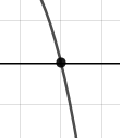
\includegraphics[width = 0.3\textwidth]{../Figures/polyZeroBehaviorAA.png}\item 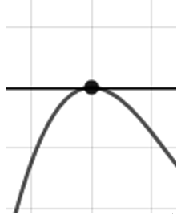
\includegraphics[width = 0.3\textwidth]{../Figures/polyZeroBehaviorBA.png}\item 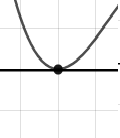
\includegraphics[width = 0.3\textwidth]{../Figures/polyZeroBehaviorCA.png}\item 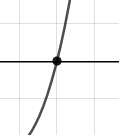
\includegraphics[width = 0.3\textwidth]{../Figures/polyZeroBehaviorDA.png}\end{multicols}\item None of the above.
\end{enumerate} }
\litem{
Construct the lowest-degree polynomial given the zeros below. Then, choose the intervals that contain the coefficients of the polynomial in the form $x^3+bx^2+cx+d$.\[ -2 + 4 i \text{ and } 4 \]\begin{enumerate}[label=\Alph*.]
\item \( b \in [0.9, 2.6], c \in [-10, -4.4], \text{ and } d \in [15, 18] \)
\item \( b \in [-3.1, 0.1], c \in [2.6, 4.7], \text{ and } d \in [79, 82] \)
\item \( b \in [0.9, 2.6], c \in [-6.7, 0.2], \text{ and } d \in [-12, -6] \)
\item \( b \in [-3.1, 0.1], c \in [2.6, 4.7], \text{ and } d \in [-82, -75] \)
\item \( \text{None of the above.} \)

\end{enumerate} }
\litem{
Which of the following equations \textit{could} be of the graph presented below?
\begin{center}
    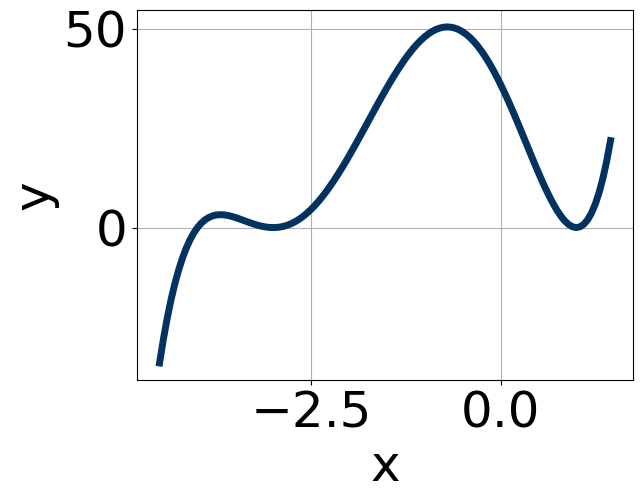
\includegraphics[width=0.5\textwidth]{../Figures/polyGraphToFunctionCopyA.png}
\end{center}
\begin{enumerate}[label=\Alph*.]
\item \( 3(x - 1)^{8} (x + 3)^{7} (x + 4)^{9} \)
\item \( 15(x - 1)^{4} (x + 3)^{8} (x + 4)^{5} \)
\item \( 13(x - 1)^{10} (x + 3)^{7} (x + 4)^{6} \)
\item \( -5(x - 1)^{6} (x + 3)^{4} (x + 4)^{4} \)
\item \( -11(x - 1)^{10} (x + 3)^{10} (x + 4)^{7} \)

\end{enumerate} }
\litem{
Describe the zero behavior of the zero $x = -5$ of the polynomial below.\[ f(x) = 6(x + 8)^{4}(x - 8)^{2}(x - 5)^{5}(x + 5)^{2} \]\begin{enumerate}[label=\Alph*.]
\begin{multicols}{2}\item 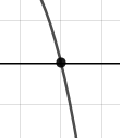
\includegraphics[width = 0.3\textwidth]{../Figures/polyZeroBehaviorCopyAA.png}\item 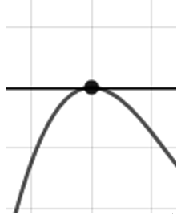
\includegraphics[width = 0.3\textwidth]{../Figures/polyZeroBehaviorCopyBA.png}\item 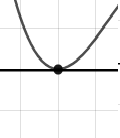
\includegraphics[width = 0.3\textwidth]{../Figures/polyZeroBehaviorCopyCA.png}\item 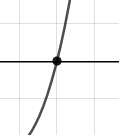
\includegraphics[width = 0.3\textwidth]{../Figures/polyZeroBehaviorCopyDA.png}\end{multicols}\item None of the above.
\end{enumerate} }
\litem{
Which of the following equations \textit{could} be of the graph presented below?
\begin{center}
    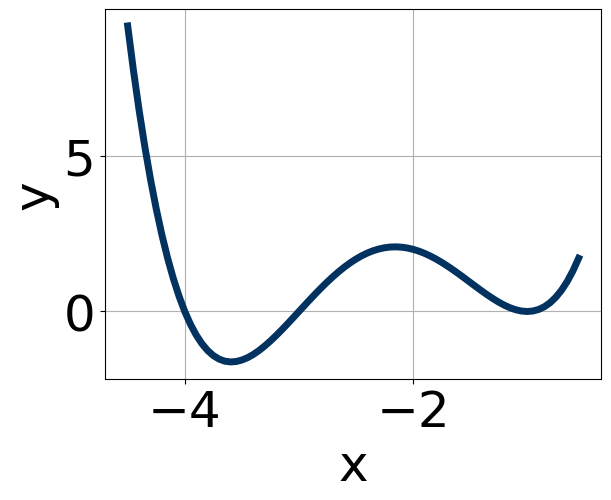
\includegraphics[width=0.5\textwidth]{../Figures/polyGraphToFunctionA.png}
\end{center}
\begin{enumerate}[label=\Alph*.]
\item \( -7(x + 1)^{6} (x + 3)^{9} (x + 4)^{7} \)
\item \( 3(x + 1)^{5} (x + 3)^{4} (x + 4)^{5} \)
\item \( 7(x + 1)^{8} (x + 3)^{9} (x + 4)^{11} \)
\item \( -7(x + 1)^{4} (x + 3)^{9} (x + 4)^{10} \)
\item \( 17(x + 1)^{6} (x + 3)^{8} (x + 4)^{5} \)

\end{enumerate} }
\litem{
Construct the lowest-degree polynomial given the zeros below. Then, choose the intervals that contain the coefficients of the polynomial in the form $x^3+bx^2+cx+d$.\[ 5 + 4 i \text{ and } 2 \]\begin{enumerate}[label=\Alph*.]
\item \( b \in [-20, -7], c \in [60, 64.2], \text{ and } d \in [-82.1, -78.6] \)
\item \( b \in [-4, 6], c \in [-9.6, -6.6], \text{ and } d \in [8.9, 14] \)
\item \( b \in [12, 16], c \in [60, 64.2], \text{ and } d \in [79, 82.4] \)
\item \( b \in [-4, 6], c \in [-6.7, -2.2], \text{ and } d \in [4.9, 9.8] \)
\item \( \text{None of the above.} \)

\end{enumerate} }
\litem{
Describe the end behavior of the polynomial below.\[ f(x) = 7(x + 8)^{4}(x - 8)^{7}(x + 3)^{3}(x - 3)^{3} \]\begin{enumerate}[label=\Alph*.]
\begin{multicols}{2}\item 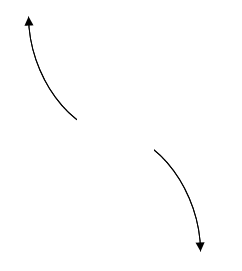
\includegraphics[width = 0.3\textwidth]{../Figures/polyEndBehaviorCopyAA.png}\item 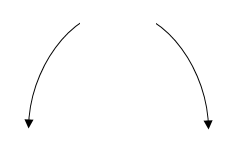
\includegraphics[width = 0.3\textwidth]{../Figures/polyEndBehaviorCopyBA.png}\item 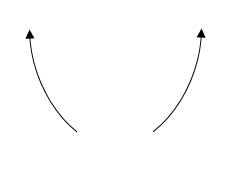
\includegraphics[width = 0.3\textwidth]{../Figures/polyEndBehaviorCopyCA.png}\item 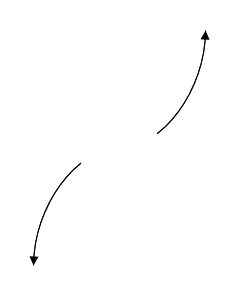
\includegraphics[width = 0.3\textwidth]{../Figures/polyEndBehaviorCopyDA.png}\end{multicols}\item None of the above.
\end{enumerate} }
\litem{
Describe the end behavior of the polynomial below.\[ f(x) = 5(x + 5)^{3}(x - 5)^{8}(x - 7)^{3}(x + 7)^{3} \]\begin{enumerate}[label=\Alph*.]
\begin{multicols}{2}\item 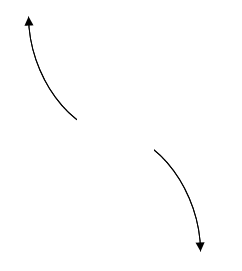
\includegraphics[width = 0.3\textwidth]{../Figures/polyEndBehaviorAA.png}\item 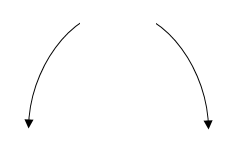
\includegraphics[width = 0.3\textwidth]{../Figures/polyEndBehaviorBA.png}\item 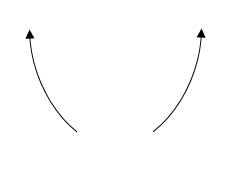
\includegraphics[width = 0.3\textwidth]{../Figures/polyEndBehaviorCA.png}\item 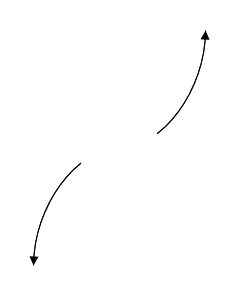
\includegraphics[width = 0.3\textwidth]{../Figures/polyEndBehaviorDA.png}\end{multicols}\item None of the above.
\end{enumerate} }
\litem{
Construct the lowest-degree polynomial given the zeros below. Then, choose the intervals that contain the coefficients of the polynomial in the form $ax^3+bx^2+cx+d$.\[ \frac{-3}{2}, \frac{-4}{3}, \text{ and } \frac{-1}{4} \]\begin{enumerate}[label=\Alph*.]
\item \( a \in [21, 26], b \in [2, 9], c \in [-61, -45], \text{ and } d \in [-12, -9] \)
\item \( a \in [21, 26], b \in [69, 75], c \in [60, 68], \text{ and } d \in [9, 16] \)
\item \( a \in [21, 26], b \in [-68, -61], c \in [27, 37], \text{ and } d \in [9, 16] \)
\item \( a \in [21, 26], b \in [69, 75], c \in [60, 68], \text{ and } d \in [-12, -9] \)
\item \( a \in [21, 26], b \in [-77, -65], c \in [60, 68], \text{ and } d \in [-12, -9] \)

\end{enumerate} }
\litem{
Construct the lowest-degree polynomial given the zeros below. Then, choose the intervals that contain the coefficients of the polynomial in the form $ax^3+bx^2+cx+d$.\[ \frac{-5}{3}, \frac{3}{5}, \text{ and } \frac{-4}{3} \]\begin{enumerate}[label=\Alph*.]
\item \( a \in [42, 46], b \in [107, 114], c \in [12, 24], \text{ and } d \in [-67, -56] \)
\item \( a \in [42, 46], b \in [-42, -40], c \in [-92, -85], \text{ and } d \in [59, 61] \)
\item \( a \in [42, 46], b \in [9, 14], c \in [-111, -107], \text{ and } d \in [-67, -56] \)
\item \( a \in [42, 46], b \in [-114, -106], c \in [12, 24], \text{ and } d \in [59, 61] \)
\item \( a \in [42, 46], b \in [107, 114], c \in [12, 24], \text{ and } d \in [59, 61] \)

\end{enumerate} }
\litem{
Describe the zero behavior of the zero $x = 6$ of the polynomial below.\[ f(x) = -3(x + 5)^{10}(x - 5)^{7}(x - 6)^{12}(x + 6)^{9} \]\begin{enumerate}[label=\Alph*.]
\begin{multicols}{2}\item 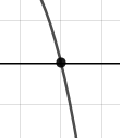
\includegraphics[width = 0.3\textwidth]{../Figures/polyZeroBehaviorAB.png}\item 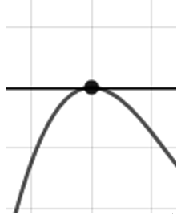
\includegraphics[width = 0.3\textwidth]{../Figures/polyZeroBehaviorBB.png}\item 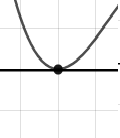
\includegraphics[width = 0.3\textwidth]{../Figures/polyZeroBehaviorCB.png}\item 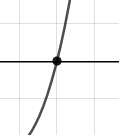
\includegraphics[width = 0.3\textwidth]{../Figures/polyZeroBehaviorDB.png}\end{multicols}\item None of the above.
\end{enumerate} }
\litem{
Construct the lowest-degree polynomial given the zeros below. Then, choose the intervals that contain the coefficients of the polynomial in the form $x^3+bx^2+cx+d$.\[ 4 - 5 i \text{ and } -2 \]\begin{enumerate}[label=\Alph*.]
\item \( b \in [1, 2], c \in [6, 8], \text{ and } d \in [9, 16] \)
\item \( b \in [6, 8], c \in [22, 31], \text{ and } d \in [-87, -77] \)
\item \( b \in [1, 2], c \in [-8, 5], \text{ and } d \in [-12, -6] \)
\item \( b \in [-6, -2], c \in [22, 31], \text{ and } d \in [75, 87] \)
\item \( \text{None of the above.} \)

\end{enumerate} }
\litem{
Which of the following equations \textit{could} be of the graph presented below?
\begin{center}
    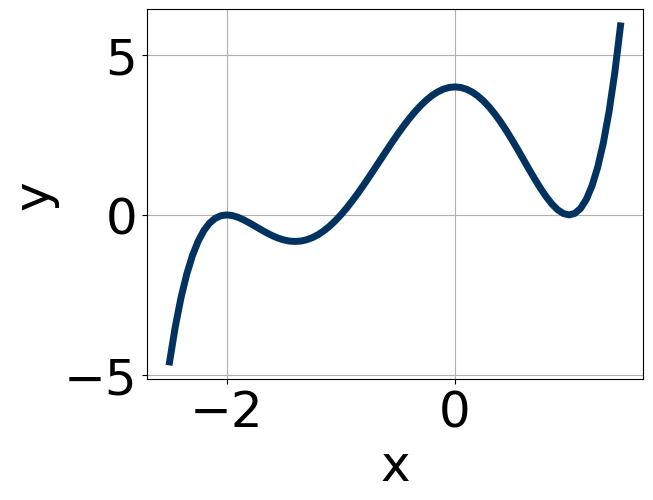
\includegraphics[width=0.5\textwidth]{../Figures/polyGraphToFunctionCopyB.png}
\end{center}
\begin{enumerate}[label=\Alph*.]
\item \( -8(x + 2)^{10} (x - 1)^{6} (x + 1)^{8} \)
\item \( 10(x + 2)^{6} (x - 1)^{6} (x + 1)^{5} \)
\item \( -15(x + 2)^{6} (x - 1)^{4} (x + 1)^{9} \)
\item \( 5(x + 2)^{10} (x - 1)^{11} (x + 1)^{7} \)
\item \( 15(x + 2)^{10} (x - 1)^{9} (x + 1)^{6} \)

\end{enumerate} }
\litem{
Describe the zero behavior of the zero $x = -6$ of the polynomial below.\[ f(x) = -9(x - 6)^{9}(x + 6)^{14}(x + 3)^{4}(x - 3)^{6} \]\begin{enumerate}[label=\Alph*.]
\begin{multicols}{2}\item 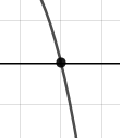
\includegraphics[width = 0.3\textwidth]{../Figures/polyZeroBehaviorCopyAB.png}\item 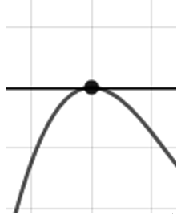
\includegraphics[width = 0.3\textwidth]{../Figures/polyZeroBehaviorCopyBB.png}\item 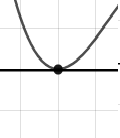
\includegraphics[width = 0.3\textwidth]{../Figures/polyZeroBehaviorCopyCB.png}\item 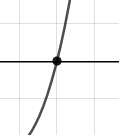
\includegraphics[width = 0.3\textwidth]{../Figures/polyZeroBehaviorCopyDB.png}\end{multicols}\item None of the above.
\end{enumerate} }
\litem{
Which of the following equations \textit{could} be of the graph presented below?
\begin{center}
    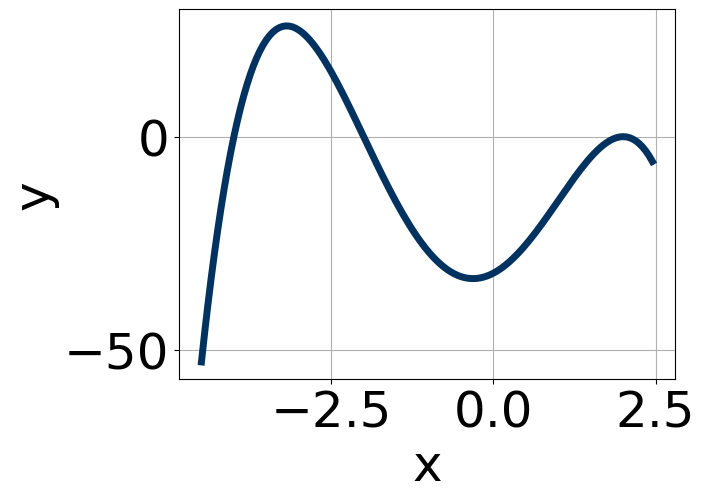
\includegraphics[width=0.5\textwidth]{../Figures/polyGraphToFunctionB.png}
\end{center}
\begin{enumerate}[label=\Alph*.]
\item \( 13(x - 2)^{8} (x + 2)^{11} (x + 4)^{10} \)
\item \( 4(x - 2)^{6} (x + 2)^{5} (x + 4)^{9} \)
\item \( -12(x - 2)^{10} (x + 2)^{8} (x + 4)^{7} \)
\item \( -14(x - 2)^{7} (x + 2)^{4} (x + 4)^{9} \)
\item \( -11(x - 2)^{6} (x + 2)^{11} (x + 4)^{7} \)

\end{enumerate} }
\litem{
Construct the lowest-degree polynomial given the zeros below. Then, choose the intervals that contain the coefficients of the polynomial in the form $x^3+bx^2+cx+d$.\[ -5 + 4 i \text{ and } -3 \]\begin{enumerate}[label=\Alph*.]
\item \( b \in [-7, 6], c \in [1, 11], \text{ and } d \in [8, 23] \)
\item \( b \in [-7, 6], c \in [-6, 2], \text{ and } d \in [-15, -11] \)
\item \( b \in [-22, -12], c \in [69, 77], \text{ and } d \in [-125, -114] \)
\item \( b \in [10, 21], c \in [69, 77], \text{ and } d \in [115, 125] \)
\item \( \text{None of the above.} \)

\end{enumerate} }
\litem{
Describe the end behavior of the polynomial below.\[ f(x) = 2(x + 9)^{3}(x - 9)^{8}(x + 5)^{3}(x - 5)^{4} \]\begin{enumerate}[label=\Alph*.]
\begin{multicols}{2}\item 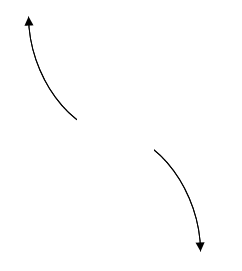
\includegraphics[width = 0.3\textwidth]{../Figures/polyEndBehaviorCopyAB.png}\item 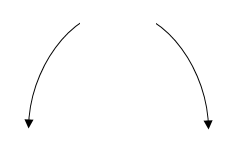
\includegraphics[width = 0.3\textwidth]{../Figures/polyEndBehaviorCopyBB.png}\item 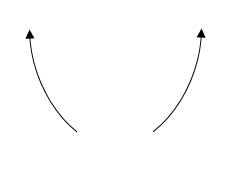
\includegraphics[width = 0.3\textwidth]{../Figures/polyEndBehaviorCopyCB.png}\item 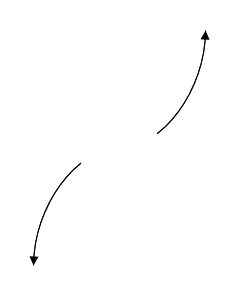
\includegraphics[width = 0.3\textwidth]{../Figures/polyEndBehaviorCopyDB.png}\end{multicols}\item None of the above.
\end{enumerate} }
\litem{
Describe the end behavior of the polynomial below.\[ f(x) = -7(x - 4)^{5}(x + 4)^{6}(x - 5)^{4}(x + 5)^{6} \]\begin{enumerate}[label=\Alph*.]
\begin{multicols}{2}\item 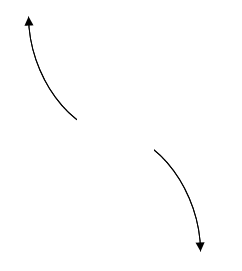
\includegraphics[width = 0.3\textwidth]{../Figures/polyEndBehaviorAB.png}\item 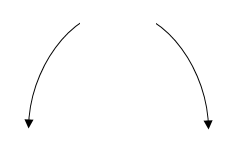
\includegraphics[width = 0.3\textwidth]{../Figures/polyEndBehaviorBB.png}\item 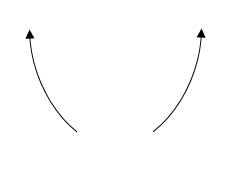
\includegraphics[width = 0.3\textwidth]{../Figures/polyEndBehaviorCB.png}\item 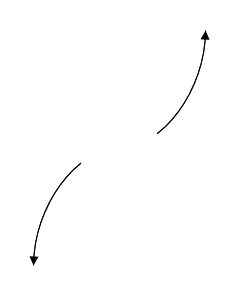
\includegraphics[width = 0.3\textwidth]{../Figures/polyEndBehaviorDB.png}\end{multicols}\item None of the above.
\end{enumerate} }
\litem{
Construct the lowest-degree polynomial given the zeros below. Then, choose the intervals that contain the coefficients of the polynomial in the form $ax^3+bx^2+cx+d$.\[ \frac{-1}{3}, 1, \text{ and } \frac{-2}{5} \]\begin{enumerate}[label=\Alph*.]
\item \( a \in [10, 17], b \in [3, 11], c \in [-9.39, -8.23], \text{ and } d \in [-0.3, 4.6] \)
\item \( a \in [10, 17], b \in [10, 23], c \in [-1.88, -0.96], \text{ and } d \in [-2.8, -0.2] \)
\item \( a \in [10, 17], b \in [-7, -3], c \in [-9.39, -8.23], \text{ and } d \in [-2.8, -0.2] \)
\item \( a \in [10, 17], b \in [-7, -3], c \in [-9.39, -8.23], \text{ and } d \in [-0.3, 4.6] \)
\item \( a \in [10, 17], b \in [-18, -11], c \in [-4.09, -2.6], \text{ and } d \in [-0.3, 4.6] \)

\end{enumerate} }
\litem{
Construct the lowest-degree polynomial given the zeros below. Then, choose the intervals that contain the coefficients of the polynomial in the form $ax^3+bx^2+cx+d$.\[ \frac{7}{3}, 1, \text{ and } \frac{-7}{2} \]\begin{enumerate}[label=\Alph*.]
\item \( a \in [0, 14], b \in [28, 31.1], c \in [12, 15], \text{ and } d \in [-57, -44] \)
\item \( a \in [0, 14], b \in [0.9, 2], c \in [-60, -55], \text{ and } d \in [-57, -44] \)
\item \( a \in [0, 14], b \in [0.9, 2], c \in [-60, -55], \text{ and } d \in [48, 54] \)
\item \( a \in [0, 14], b \in [40.6, 41.8], c \in [82, 89], \text{ and } d \in [48, 54] \)
\item \( a \in [0, 14], b \in [-4.2, 0.2], c \in [-60, -55], \text{ and } d \in [-57, -44] \)

\end{enumerate} }
\litem{
Describe the zero behavior of the zero $x = -4$ of the polynomial below.\[ f(x) = -4(x + 4)^{5}(x - 4)^{8}(x - 9)^{3}(x + 9)^{4} \]\begin{enumerate}[label=\Alph*.]
\begin{multicols}{2}\item 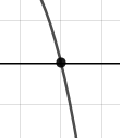
\includegraphics[width = 0.3\textwidth]{../Figures/polyZeroBehaviorAC.png}\item 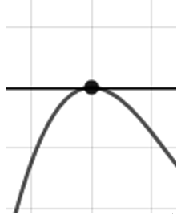
\includegraphics[width = 0.3\textwidth]{../Figures/polyZeroBehaviorBC.png}\item 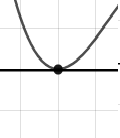
\includegraphics[width = 0.3\textwidth]{../Figures/polyZeroBehaviorCC.png}\item 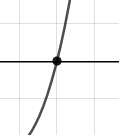
\includegraphics[width = 0.3\textwidth]{../Figures/polyZeroBehaviorDC.png}\end{multicols}\item None of the above.
\end{enumerate} }
\litem{
Construct the lowest-degree polynomial given the zeros below. Then, choose the intervals that contain the coefficients of the polynomial in the form $x^3+bx^2+cx+d$.\[ 5 - 2 i \text{ and } 1 \]\begin{enumerate}[label=\Alph*.]
\item \( b \in [-14, -9], c \in [37, 44], \text{ and } d \in [-34, -23] \)
\item \( b \in [2, 13], c \in [37, 44], \text{ and } d \in [27, 33] \)
\item \( b \in [-2, 6], c \in [-2, 5], \text{ and } d \in [-6, 1] \)
\item \( b \in [-2, 6], c \in [-6, -5], \text{ and } d \in [0, 8] \)
\item \( \text{None of the above.} \)

\end{enumerate} }
\litem{
Which of the following equations \textit{could} be of the graph presented below?
\begin{center}
    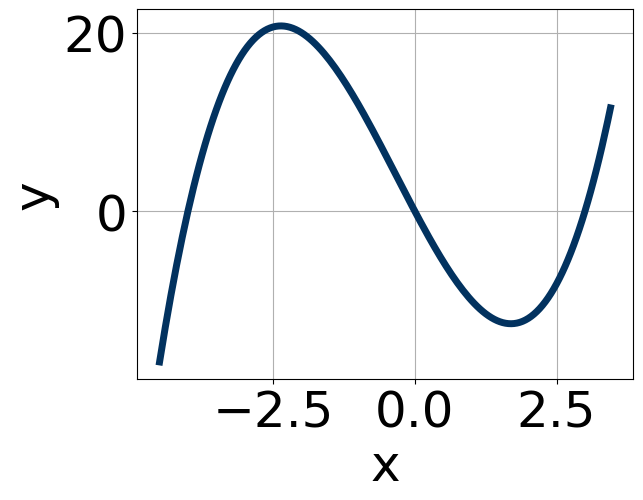
\includegraphics[width=0.5\textwidth]{../Figures/polyGraphToFunctionCopyC.png}
\end{center}
\begin{enumerate}[label=\Alph*.]
\item \( -11x^{6} (x + 4)^{11} (x - 3)^{5} \)
\item \( 7x^{9} (x + 4)^{11} (x - 3)^{9} \)
\item \( -6x^{7} (x + 4)^{5} (x - 3)^{5} \)
\item \( 6x^{8} (x + 4)^{4} (x - 3)^{11} \)
\item \( 8x^{8} (x + 4)^{5} (x - 3)^{7} \)

\end{enumerate} }
\litem{
Describe the zero behavior of the zero $x = -8$ of the polynomial below.\[ f(x) = 4(x - 7)^{5}(x + 7)^{3}(x + 8)^{9}(x - 8)^{8} \]\begin{enumerate}[label=\Alph*.]
\begin{multicols}{2}\item 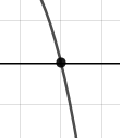
\includegraphics[width = 0.3\textwidth]{../Figures/polyZeroBehaviorCopyAC.png}\item 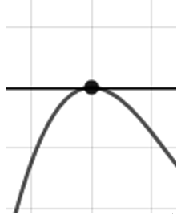
\includegraphics[width = 0.3\textwidth]{../Figures/polyZeroBehaviorCopyBC.png}\item 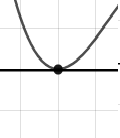
\includegraphics[width = 0.3\textwidth]{../Figures/polyZeroBehaviorCopyCC.png}\item 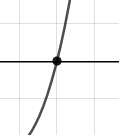
\includegraphics[width = 0.3\textwidth]{../Figures/polyZeroBehaviorCopyDC.png}\end{multicols}\item None of the above.
\end{enumerate} }
\litem{
Which of the following equations \textit{could} be of the graph presented below?
\begin{center}
    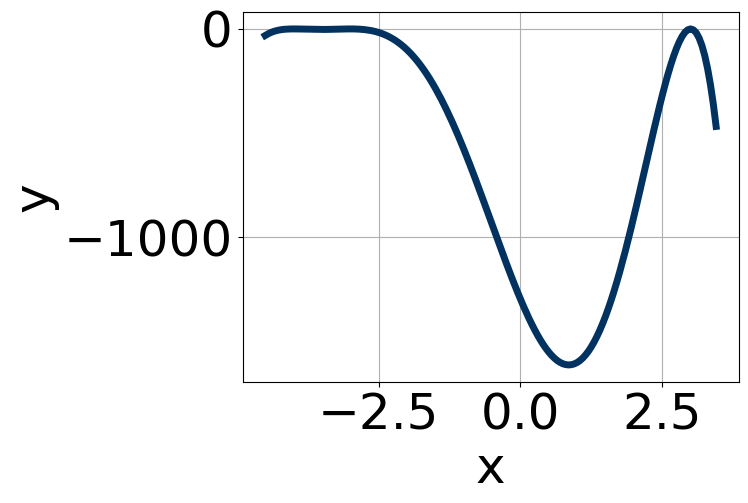
\includegraphics[width=0.5\textwidth]{../Figures/polyGraphToFunctionC.png}
\end{center}
\begin{enumerate}[label=\Alph*.]
\item \( 16(x + 4)^{10} (x - 3)^{10} (x + 3)^{6} \)
\item \( -4(x + 4)^{4} (x - 3)^{10} (x + 3)^{4} \)
\item \( 14(x + 4)^{10} (x - 3)^{4} (x + 3)^{11} \)
\item \( -7(x + 4)^{4} (x - 3)^{11} (x + 3)^{7} \)
\item \( -10(x + 4)^{10} (x - 3)^{6} (x + 3)^{11} \)

\end{enumerate} }
\litem{
Construct the lowest-degree polynomial given the zeros below. Then, choose the intervals that contain the coefficients of the polynomial in the form $x^3+bx^2+cx+d$.\[ 5 - 2 i \text{ and } 4 \]\begin{enumerate}[label=\Alph*.]
\item \( b \in [-17, -13], c \in [69, 79], \text{ and } d \in [-116, -115] \)
\item \( b \in [-7, 5], c \in [-5, 6], \text{ and } d \in [-9, -2] \)
\item \( b \in [-7, 5], c \in [-13, -6], \text{ and } d \in [10, 27] \)
\item \( b \in [14, 16], c \in [69, 79], \text{ and } d \in [114, 119] \)
\item \( \text{None of the above.} \)

\end{enumerate} }
\litem{
Describe the end behavior of the polynomial below.\[ f(x) = -9(x + 2)^{4}(x - 2)^{5}(x - 6)^{5}(x + 6)^{7} \]\begin{enumerate}[label=\Alph*.]
\begin{multicols}{2}\item 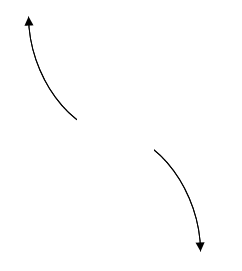
\includegraphics[width = 0.3\textwidth]{../Figures/polyEndBehaviorCopyAC.png}\item 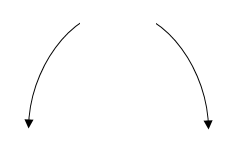
\includegraphics[width = 0.3\textwidth]{../Figures/polyEndBehaviorCopyBC.png}\item 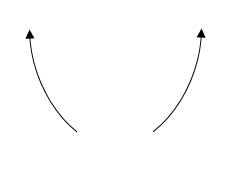
\includegraphics[width = 0.3\textwidth]{../Figures/polyEndBehaviorCopyCC.png}\item 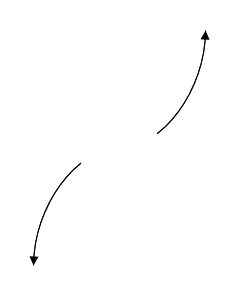
\includegraphics[width = 0.3\textwidth]{../Figures/polyEndBehaviorCopyDC.png}\end{multicols}\item None of the above.
\end{enumerate} }
\litem{
Describe the end behavior of the polynomial below.\[ f(x) = 9(x + 3)^{2}(x - 3)^{3}(x - 4)^{4}(x + 4)^{5} \]\begin{enumerate}[label=\Alph*.]
\begin{multicols}{2}\item \includegraphics[width = 0.3\textwidth]{../Figures/polyEndBehaviorAC.png}\item \includegraphics[width = 0.3\textwidth]{../Figures/polyEndBehaviorBC.png}\item \includegraphics[width = 0.3\textwidth]{../Figures/polyEndBehaviorCC.png}\item \includegraphics[width = 0.3\textwidth]{../Figures/polyEndBehaviorDC.png}\end{multicols}\item None of the above.
\end{enumerate} }
\litem{
Construct the lowest-degree polynomial given the zeros below. Then, choose the intervals that contain the coefficients of the polynomial in the form $ax^3+bx^2+cx+d$.\[ \frac{-7}{4}, \frac{-7}{5}, \text{ and } 4 \]\begin{enumerate}[label=\Alph*.]
\item \( a \in [20, 23], b \in [-144, -139], c \in [301, 307], \text{ and } d \in [-196, -195] \)
\item \( a \in [20, 23], b \in [9, 18], c \in [-207, -199], \text{ and } d \in [189, 200] \)
\item \( a \in [20, 23], b \in [-19, -15], c \in [-207, -199], \text{ and } d \in [-196, -195] \)
\item \( a \in [20, 23], b \in [-92, -78], c \in [-26, -20], \text{ and } d \in [189, 200] \)
\item \( a \in [20, 23], b \in [-19, -15], c \in [-207, -199], \text{ and } d \in [189, 200] \)

\end{enumerate} }
\end{enumerate}

\end{document}